% =============================================================================
% APA 7th Edition Formatted Paper
% Uses: apa7 conventions via apacite + natbibapa
% =============================================================================
\documentclass[12pt]{article}

% ----- Page Layout (APA: 1-inch margins) -----
\usepackage[margin=1in,headheight=14.5pt]{geometry}
\addtolength{\topmargin}{-2.5pt}

% ----- Typography (APA: Times New Roman or similar serif) -----
\usepackage{newtxtext,newtxmath}
\usepackage[T1]{fontenc}
% Reset typewriter font to avoid missing t1xtt error when apacite renders URLs
\renewcommand{\ttdefault}{cmtt}
% url package: allow line breaks in bibliography URLs (must come before apacite)
\usepackage[hyphens]{url}

% ----- Spacing (APA: double-spaced throughout) -----
\usepackage{setspace}
\doublespacing

% ----- Headers (APA 7th Student Paper: page number only, no running head) -----
\usepackage{fancyhdr}
\pagestyle{fancy}
\fancyhf{}
\renewcommand{\headrulewidth}{0pt}
\fancyhead[R]{\thepage}

% ----- References: apacite must be loaded BEFORE hyperref -----
\usepackage[natbibapa]{apacite}
\bibliographystyle{apacite}
\shortcites{ref2,ref3,ref4,ref5,ref6,ref7,ref8,ref9,ref11,ref12,ref13,ref14,ref15,ref16,ref17,ref18,ref19,ref21,ref22,ref23,ref24,ref25,ref26,ref27,ref28,ref29,ref30,ref31,ref33,ref34,ref35,ref36,ref37,chawla2002smote,batista2004study,chen2016xgboost,ke2017lightgbm,breiman2001random,friedman2001greedy,lundberg2017unified,tolles2016logistic,who2023tb,sibanda2026explainable,asad2020framework,salmi2024imbalanced,hastie2009elements,nishat2022smoteenn}

% ----- Hyperlinks (loaded after apacite to avoid citation link conflicts) -----
\usepackage{hyperref}
\hypersetup{
  colorlinks=true,
  linkcolor=black,
  citecolor=black,
  urlcolor=blue
}

% ----- Figures & Tables -----
\usepackage{graphicx}
\usepackage{float}
\usepackage{tikz}
\usetikzlibrary{shapes.geometric,arrows.meta,positioning}
\usepackage{booktabs}
\usepackage{pdfpages}
\usepackage{caption}
\usepackage{placeins}
% APA: table/figure captions are bold label, newline, then italic title
\captionsetup{labelsep=newline, justification=raggedright, singlelinecheck=false, font=doublespacing, labelfont=bf, textfont=it}

% ----- Section Formatting (APA 7th Heading Levels) -----
\usepackage{etoolbox}

% Level 1: Centered, Bold, Title Case
\makeatletter
\renewcommand{\section}{\@startsection{section}{1}{0pt}%
  {1.5\baselineskip plus 0.2\baselineskip minus 0.1\baselineskip}%
  {0.5\baselineskip}%
  {\centering\bfseries\normalsize}}

% Level 2: Left-Aligned, Bold, Title Case
\renewcommand{\subsection}{\@startsection{subsection}{2}{0pt}%
  {1.5\baselineskip plus 0.2\baselineskip minus 0.1\baselineskip}%
  {0.5\baselineskip}%
  {\bfseries\normalsize}}

% Level 3: Left-Aligned, Bold Italic, Title Case
\renewcommand{\subsubsection}{\@startsection{subsubsection}{3}{0pt}%
  {1.5\baselineskip plus 0.2\baselineskip minus 0.1\baselineskip}%
  {0.5\baselineskip}%
  {\bfseries\itshape\normalsize}}
\makeatother

% ----- Suppress section numbering (APA uses formatting, not numbers) -----
\setcounter{secnumdepth}{0}

% ----- Paragraph formatting (APA: 0.5-inch indent, no extra space between paragraphs) -----
\setlength{\parindent}{0.5in}
\setlength{\parskip}{0pt}

% Ensure enumerate and itemize have no extra spacing
\usepackage{enumitem}
\setlist{nosep, leftmargin=0.5in}

% =============================================================================
\begin{document}

% ======================== TITLE PAGE (APA 7th Student Paper) ========================
\begin{center}
\vspace*{3\baselineskip}

{\bfseries Treatment Success and Failure Prediction Using Machine Learning Models\\
for Pulmonary Tuberculosis Patients Under the Department of Health-Cordillera Administrative Region (DOH-CAR) Tuberculosis-Directly Observed Treatment, Short-course (TB-DOTS) Program}

\vspace{2\baselineskip}

Aaron Kyle M. Aguilar, Mark Lestat C. Agustin, Keanu Sonn M. Fortaleza,\\
Benny Gil A. Lactaotao, Marven Joffre G. Luis, Georcelle Leisley U. Nuarin,\\
Sean Drei A. Octavo, and Gebreyl Isaac P. Rabang

\vspace{0.5\baselineskip}

Department of Computing and Information Studies, Saint Louis University

% ----- Author Note (commented out for now) -----
% \vspace{0.5\baselineskip}
% TODO: Replace with your actual course number and name
% COURSE NUMBER: Course Name
% Josephine S. Dela Cruz, DIT
% \vspace{0.5\baselineskip}
% April 24, 2026

\end{center}

\newpage

% ======================== ABSTRACT ========================
% APA 7th: "Abstract" centered, bold; abstract text is NOT indented (no \parindent)
\begin{center}
\textbf{Abstract}
\end{center}

% APA 7th: Abstract is a single unindented paragraph
{\setlength{\parindent}{0pt}
Pulmonary Tuberculosis (PTB) remains a critical public health challenge in the Cordillera Administrative Region (CAR), Philippines, where complex patient profiles and programmatic gaps contribute to persistent treatment failure. This study develops machine learning models to predict treatment success or failure among PTB patients in DOH-CAR TB-DOTS facilities covering the period 2015--2025. A standardized preprocessing pipeline performs schema harmonization, patient pseudonymization, and a diagnostic-first missing data handling protocol that classifies each variable's missingness mechanism---Missing Completely at Random (MCAR), Missing at Random (MAR), or Missing Not at Random (MNAR)---before routing it to one of four targeted strategies: column exclusion, listwise deletion, missing indicator imputation, or stochastic Multivariate Imputation by Chained Equations (MICE). Supervised models---Logistic Regression, Support Vector Machines (SVM), and Extreme Gradient Boosting (XGBoost)---are trained alongside Recurrent Neural Network (RNN) and Long Short-Term Memory (LSTM) temporal architectures to capture longitudinal treatment dynamics across the 6- to 12-month treatment course. Shapley Additive Explanations (SHAP) ensure model interpretability by quantifying the contribution of individual patient features to each prediction. The validated models are embedded in a Clinical Decision Support System (CDSS) that provides dynamic risk estimates and factor-level explanations to support early clinical intervention for patients at risk of treatment failure.

% APA 7th: Keywords line is NOT indented; label is italic
\textit{Keywords:} tuberculosis, machine learning, treatment outcome prediction, clinical decision support system, explainable AI
}

\newpage

% ======================== BODY ========================
\newpage
\begin{center}
{\bfseries Treatment Success and Failure Prediction Using Machine Learning Models\\
for Pulmonary Tuberculosis Patients Under the Department of Health-Cordillera Administrative Region (DOH-CAR) Tuberculosis-Directly Observed Treatment, Short-course (TB-DOTS) Program}
\end{center}

Pulmonary Tuberculosis (PTB) is a chronic infectious disease caused by \textit{Mycobacterium tuberculosis} (MTB), a slow-growing and acid-fast bacillus that continues to challenge public health due to its gradual progression and risk of treatment failure \citep{ref20}. Despite effective therapies, PTB remains widespread due to its strong association with poverty, undernutrition, and comorbidities such as diabetes and HIV which weaken immune defenses and increase susceptibility \citep{ref20}. These factors delay diagnosis, complicate treatment, and contribute to disease progression. Globally, TB is still one of the leading causes of death, with 1.5 million deaths and 10 million new cases recorded in 2018, including half a million with rifampicin resistance.

In the Philippines, TB continues to be a major public health concern. The World Health Organization (WHO) identifies the country as one of the top contributors to the global TB burden as it accounts for an estimated 6.8 percent of cases. Before the COVID-19 pandemic, the Philippines had one of the highest TB rates in Asia with over 554 cases per 100,000 people in 2019 \citep{ref8}. In 2023, around 37,000 Filipinos died from TB out of the 739,000 diagnosed cases. The WHO classifies the country as a high burden for MDR-TB and TB/HIV co-infection \citep{ref18}. That same year, the DOH recorded 575,770 TB cases through its Integrated TB Information System which indicates that many cases remain unregistered or undiagnosed \citep{ref4}. The DOH implements CDC-recommended regimens for active and latent TB through the TB-DOTS strategy which was expanded in 2003 to include private clinics, pharmacies, and hospitals \citep{ref5, ref6}. Despite these initiatives, gaps in diagnosis, treatment monitoring, and patient support persist especially in the management of MDR-TB \citep{ref29}.

In Baguio City, the DOH-CAR reported 437 confirmed TB cases in 2022 along with over 4,405 missing or unreported cases making the area a priority for surveillance and treatment improvement \citep{ref25}. Contributing factors include high population density, internal migration, climate, and the city's role as a referral center for nearby provinces. Patient comorbidities, socioeconomic barriers, and health system limitations also influence treatment outcomes \citep{ref30}. These challenges highlight the need for locally adaptive strategies as treatment failure not only worsens patient outcomes but also prolongs transmission and drives the emergence of MDR-TB \citep{ref28}.

\subsection{Risk Factors for Treatment Failure}

To ensure uniformity in the evaluation of TB control efforts, the DOH has established standardized criteria for classifying treatment outcomes through the National Tuberculosis Program (NTP). Establishing these outcomes is crucial for monitoring program performance, ensuring comparability across studies, and informing risk factor analysis. Ultimately, these outcomes of success or failure are not random but are linked to a distinct set of patient-specific, clinical, and programmatic risk factors. While mortality remains the primary outcome for most studies on treatment failure, some also consider the development of disease, resistance to multiple anti-TB drugs, and failure to follow up \citep{ref6}.

One of the risk factors is that TB patients have close contact with other patients with active TB infection. A study noted that TB patients who acquired the infection through close contact were shown to be at higher risk of delayed diagnosis and more likely to be non-adherent with the treatment either by refusing or discontinuing the regimen \citep{ref7}. Another risk factor is recurrence of the infection or having a history of receiving TB treatment. TB patients who missed follow-ups had a higher risk of reactivation of the infection and mortality as they are more difficult to treat compared to patients with no prior history of TB \citep{ref21}. Furthermore, missed or interrupted treatment causes the development of resistance to the drug if done frequently \citep{ref13}.

Comorbidities are also discussed in studies that have consistently shown a significant influence on tuberculosis treatment outcomes across different settings. In Eastern Ethiopia, HIV co-infection was determined to be a substantial risk factor for treatment failure due to the weakened immune system which leads to a higher risk for ineffective treatment \citep{ref2}. In addition, TB and HIV drug interactions accelerate each other's progression and increase the occurrence of side effects or adverse effects which may compromise treatment success \citep{ref3}. Likewise, a study in Davao City, Philippines, revealed that there was a higher risk of treatment failure in comorbid patients with 58.82\% of the 51 patients who experienced treatment failure having at least one comorbidity \citep{ref9}. Another major determinant is Diabetes Mellitus (DM). TB patients with diagnosed DM have a higher risk of treatment failure, relapse, and death compared to non-diabetics \citep{ref14}. In a systematic review and meta-analysis, patients with DM have a higher risk of experiencing treatment failure for Drug-resistant (DR) and mortality for MDR-TB with an odds ratio of 1.56 and 1.57 respectively \citep{ref22}. In line with this, another study states that patients suffering from both PTB and chronic conditions, particularly DM, had reduced rates of sputum conversion with a higher probability of poor treatment outcomes including death and progression to MDR-TB \citep{ref17}.

\subsection{Machine Learning for TB Outcome Prediction}

Although multiple studies have examined risk factors such as sociodemographic characteristics, comorbidities, and medical history, the findings remain inconsistent and fragmented since methodological constraints limit them. Most studies rely on traditional statistical analyses which are statistical tests or regressions that examine one factor at a time or a few factors together while assuming their linear relationships \citep{ref2}. These limitations highlight the need for an integrative approach to combine multiple dimensions of data in analyzing the interrelated variables together as a critical gap in capturing the multifaceted nature of TB treatment outcomes.

To address this gap, the present study adopts a holistic multi-layer analytical framework that integrates descriptive analysis and supervised predictive modeling using demographic, clinical, diagnostic, and treatment-related variables. Descriptive analyses are employed to characterize patient profiles and treatment patterns, while supervised learning models are used to predict treatment outcomes. This integrative approach enables machine learning models to learn complex relationships among multiple patient-level variables that influence treatment success or failure, thereby enhancing both predictive accuracy and interpretability \citep{ref23, ref24}.

Machine learning (ML) offers a distinct advantage in modeling complex and non-linear interactions among demographic, clinical, diagnostic, and treatment-related variables that conventional statistical analyses may overlook. By leveraging algorithms capable of learning from high-dimensional data, such as logistic regression, Support Vector Machines (SVM), and ensemble-based methods including Extreme Gradient Boosting (XGBoost), the study aims to uncover subtle dependencies that contribute to treatment success or failure \citep{ref16}. Previous research has demonstrated the utility of ML in TB research, including predicting drug resistance, identifying high-risk patients, and optimizing treatment strategies \citep{ref26, ref27, sibanda2026explainable, asad2020framework}. In this study, the models are trained directly on integrated patient data, allowing them to capture individual-level patterns that improve predictive performance while maintaining interpretability.

Beyond prediction, interpretability will be enhanced through the application of Shapley Additive Explanations (SHAP) which is a post-hoc interpretability technique that quantifies the contribution of each variable to the model's predictions. SHAP enables a transparent evaluation of which patient features most strongly drive treatment success or failure. This supports explainable and trustworthy Artificial Intelligence (AI) in clinical contexts \citep{ref15}. Using supervised learning with interpretable AI methods, this framework not only forecasts treatment outcomes but also reveals the relative importance of risk factors such as drug resistance, comorbidities, or regimen adherence. The resulting models are designed to help healthcare providers identify patients at a higher risk of treatment failure thus enabling early intervention, tailored regimens, and improved patient management.

\subsection{Contributions}

The main contributions of this paper are as follows:

\begin{enumerate}
\item \textbf{Integrated Predictive Framework.} The team develop and validate machine learning models that accurately predict therapy success or failure among TB patients in the CAR, Philippines. The integration of demographic, clinical, and laboratory variables focuses on supporting early identification of patients at risk of unsuccessful treatment and providing evidence-based tools for improving TB program outcomes.
\item \textbf{Data Preprocessing and Harmonization.} The team pre-process and document patient records of PTB cases from TB-DOTS facilities in the CAR through data cleaning, feature engineering, and reporting for readiness to be used in ML applications.
\item \textbf{Descriptive and Exploratory Analysis.} The team analyzed the demographic, clinical, diagnostic, and treatment characteristics of PTB patients to provide a comprehensive overview of the study population and identify key variables associated with treatment outcomes over the course of therapy.
\item \textbf{Temporal Modeling.} The team incorporates temporal modeling that analyzes time-dependent patterns in patient data allowing the detection of dynamic changes and trends throughout treatment. This thereby improves the accuracy of outcome predictions and supports timely clinical interventions.
\item \textbf{Clinical Decision Support.} The team developed a decision support tool that visualizes patient risk levels and predictive outputs. This enables early identification of individuals at risk of poor outcomes and ensures that the model maintains high predictive accuracy and reliability when applied to evaluate incoming TB cases.
\end{enumerate}

\subsection{Research Objectives}

This study aims to develop and validate machine learning models that accurately predict therapy success or failure among TB patients in the CAR, Philippines. The integration of demographic, clinical, and laboratory variables focuses on supporting early identification of patients at risk of unsuccessful treatment and providing evidence-based tools for improving TB program outcomes, with the overarching goal of enabling personalized clinical interventions and efficient allocation of healthcare resources. Specifically, the research aims to achieve the following objectives:

\begin{enumerate}
    \item To pre-process and document patient records of PTB cases from TB-DOTS facilities in the CAR through data cleaning, feature engineering, and reporting for readiness to be used in ML applications.
    \item To describe the demographic, clinical, diagnostic, and treatment characteristics of PTB patients in the dataset, providing an overview of the study population.
    \item To identify contributing variables that influence treatment outcomes over the course of therapy, enabling recognition of the most critical factors that affect patient recovery and guiding more precise treatment adjustments that can be intervened with.
    \item To incorporate temporal modeling that analyzes time-dependent patterns in patient data, allowing the detection of dynamic changes and trends throughout treatment, thereby improving the accuracy of outcome predictions and supporting timely clinical interventions.
    \item To train and validate supervised learning models for predicting treatment success or failure among PTB patients, enabling early identification of individuals at risk of poor outcomes and ensuring that the model maintains high predictive accuracy and reliability when applied to evaluate incoming TB cases.
    \item To develop a decision support tool that visualizes patient risk levels and predictive outputs.
\end{enumerate}

\subsection{Scope and Limitations}

The dataset will include PTB patients for the period 2015--2025 in the CAR excluding those who are still undergoing treatment at the time of data extraction. Furthermore, only patients with a well-defined treatment outcome of either success or failure will be included. The data gathered will encompass demographic information, laboratory tests, diagnostic data, clinical data, treatment regimen, follow-up examinations, drug administration data, and treatment outcomes. The study faces limitations related to the sufficiency and quality of the dataset. The data sourced from existing records may present challenges related to completeness, consistency, and representativeness due to limited access to complete clinical parameters. This could affect the inclusion of important risk factors and weaken the robustness of the analysis. Additionally, the study may not fully represent the current TB patient population as patients currently undergoing treatment are excluded. Difficulties are also expected during data extraction from DOH-CAR as variations in record-keeping over the 10-year period from 2015 to 2025 may be inconsistent due to changes in the healthcare system and shifts in documentation standards. Reliance on self-reported indicators may also introduce bias and inconsistencies that could affect the predictive capabilities of the model.

\subsection{Significance of the Study}

The resulting models are designed to help healthcare providers identify patients at a higher risk of treatment failure thus enabling early intervention, tailored regimens, and improved patient management. Ultimately, this machine learning framework supports the broader objective of strengthening TB control efforts in the Cordillera Administrative Region (CAR) by transforming existing patient data into predictive, explainable, and actionable tools for evidence-based public health practice. The results will help improve patient management and treatment planning, strengthen program implementation, and guide public health decision-making to improve the TB treatment success rate in CAR. Furthermore, the study aims to maximize benefits for the public by informing health administrators about the model which may be further developed into a solution or application to aid the local TB-DOTS program. The processed and pseudonymized derivative of the DOH-CAR PTB Treatment Outcome Dataset produced by the study will also be published to support the advancement of clinical, epidemiological, and machine learning research.

% ======================== METHOD ========================
\section{Method}

This study uses a dataset of records of PTB patients from the Cordillera Administrative Region (CAR), Philippines, covering 2015--2025 and consolidated by the Department of Health--CAR (DOH-CAR). After ethical approval, records are pseudonymized and processed using a standardized preprocessing pipeline, including schema harmonization, error correction, and feature scaling, followed by a diagnostic-first missing data handling protocol described in the Missing Data Handling subsection below. Exploratory and cluster analyses are conducted to characterize the cohort and derive subgroup-level features. Supervised models, Logistic Regression, Support Vector Machines (SVM), and Extreme Gradient Boosting (XGBoost), are trained to predict treatment outcomes defined by National Tuberculosis Program criteria. To capture longitudinal treatment dynamics, temporal models using Recurrent Neural Networks (RNN) and Long Short-Term Memory (LSTM) are evaluated alongside static models, with ensemble strategies applied for improved robustness. Model performance is assessed using standard classification metrics, and Shapley Additive Explanations (SHAP) are employed to ensure interpretability. The final models are integrated into a clinical decision support framework to provide dynamic risk estimates throughout the treatment course. An overview can be found in Figure~\ref{fig:data_management}.

\begin{figure}[p]
\caption{Data Management and Analysis Process}
\label{fig:data_management}
\centering
\resizebox{\columnwidth}{!}{%
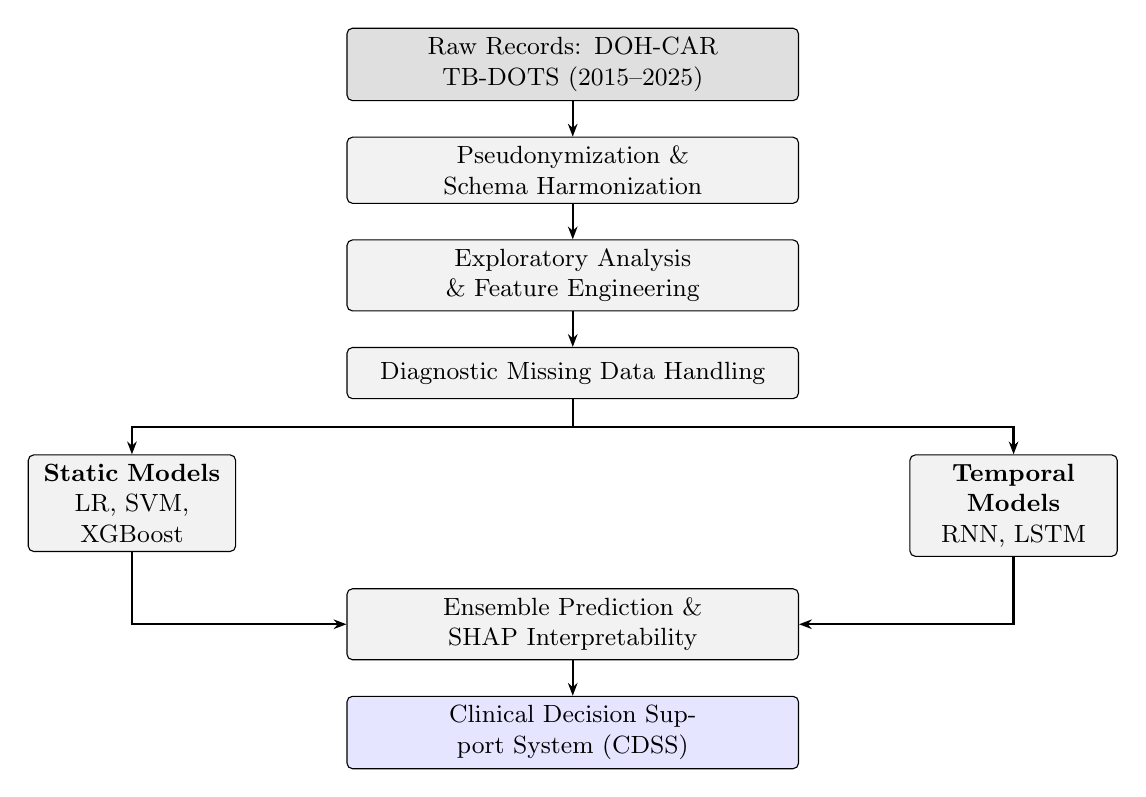
\begin{tikzpicture}[
  node distance=0.45cm and 0.6cm,
  mainbox/.style={rectangle, draw, rounded corners=2pt, text width=5.5cm,
    minimum height=0.65cm, align=center, font=\small, fill=gray!10},
  splitbox/.style={rectangle, draw, rounded corners=2pt, text width=2.4cm,
    minimum height=0.65cm, align=center, font=\small, fill=gray!10},
  arrow/.style={-{Stealth[scale=0.7]}, thick}
]
  \node[mainbox, fill=gray!25] (raw)      {Raw Records: DOH-CAR TB-DOTS (2015--2025)};
  \node[mainbox, below=of raw]  (harm)    {Pseudonymization \& Schema Harmonization};
  \node[mainbox, below=of harm] (eda)     {Exploratory Analysis \& Feature Engineering};
  \node[mainbox, below=of eda]  (mdh)     {Diagnostic Missing Data Handling};
  \node[splitbox, below left=0.7cm and 1.4cm of mdh]  (static)   {\textbf{Static Models}\\LR, SVM, XGBoost};
  \node[splitbox, below right=0.7cm and 1.4cm of mdh] (temporal)  {\textbf{Temporal Models}\\RNN, LSTM};
  \node[mainbox, below=2.4cm of mdh]  (shap)  {Ensemble Prediction \& SHAP Interpretability};
  \node[mainbox, below=of shap, fill=blue!10] (cdss) {Clinical Decision Support System (CDSS)};
  \draw[arrow] (raw)  -- (harm);
  \draw[arrow] (harm) -- (eda);
  \draw[arrow] (eda)  -- (mdh);
  \draw[arrow] (mdh.south) -- ++(0,-0.35) -| (static.north);
  \draw[arrow] (mdh.south) -- ++(0,-0.35) -| (temporal.north);
  \draw[arrow] (static.south)   |- (shap.west);
  \draw[arrow] (temporal.south) |- (shap.east);
  \draw[arrow] (shap) -- (cdss);
\end{tikzpicture}%
}
\end{figure}

\FloatBarrier

\subsection{Data Acquisition and Preprocessing}

The study utilizes a retrospective dataset of PTB patients from the Cordillera Administrative Region (CAR), Philippines, covering the period from 2015 to 2025. Data is centrally consolidated by the Department of Health-CAR (DOH-CAR), which manages reports from government TB-DOTS facilities and private practitioners under the Public-Private Mix DOTS (PPMD) scheme \citep{ref6}.

The raw dataset comprises demographic variables (e.g., age, sex, civil status), clinical indicators (e.g., BMI, blood pressure), and diagnostic results (e.g., GeneXpert, Smear Microscopy). To ensure data quality for machine learning applications, a reproducible preprocessing pipeline is implemented. This includes schema harmonization to standardize variable formats and units, and the removal of direct identifiers to strictly enforce patient privacy. Missing data, a common challenge in clinical registries, is addressed through a diagnostic-first protocol described in the Missing Data Handling subsection below.

\subsection{Exploratory Data Analysis}

Prior to predictive modeling, an exploratory analysis is conducted to characterize the study population and identify latent subgroups. The study employs cluster analysis on demographic, clinical, and diagnostic dimensions to detect natural groupings of patients. These clusters reveal distinguishing features such as specific comorbidity profiles, adherence behaviors, and regimen responses. Importantly, the resulting cluster assignments are not merely descriptive; they are integrated as engineered features into the subsequent supervised learning models. This approach enables the algorithms to learn both individual-level attributes and subgroup-level patterns that significantly influence treatment success or failure.

\subsection{Missing Data Handling}

Clinical TB registries exhibit heterogeneous missingness arising from inconsistent documentation, varying facility capacities, and the longitudinal structure of treatment monitoring. Applying a single imputation strategy uniformly across all variables is statistically inappropriate when the mechanism generating missingness differs across features. Accordingly, this study implements a diagnostic-first missing data pipeline that first classifies each variable's missingness mechanism and then routes the variable to one of four handling strategies: column exclusion, listwise deletion, missing indicator with fill, or stochastic Multiple Imputation by Chained Equations (MICE) imputation (Figure~\ref{fig:missing_data_pipeline}) \citep{ref31, ref32}.

\begin{figure}[p]
\centering
\resizebox{\columnwidth}{!}{%
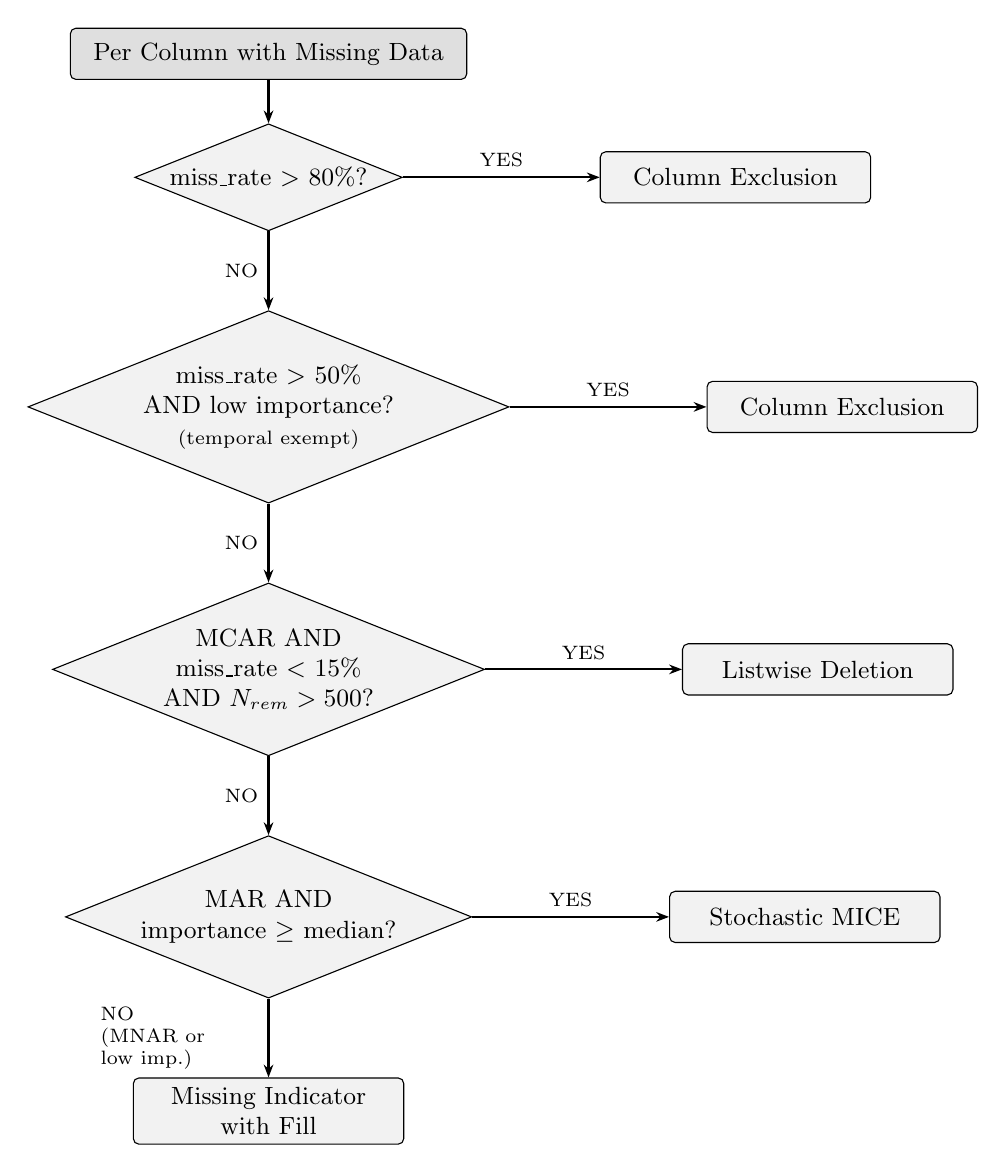
\begin{tikzpicture}[
  node distance=0.55cm and 0.8cm,
  mainbox/.style={rectangle, draw, rounded corners=2pt, text width=4.8cm,
    minimum height=0.65cm, align=center, font=\small, fill=gray!10},
  decision/.style={diamond, draw, aspect=2.5, inner sep=1pt,
    align=center, font=\small, fill=gray!10},
  outcome/.style={rectangle, draw, rounded corners=2pt, text width=3.2cm,
    minimum height=0.65cm, align=center, font=\small, fill=gray!10},
  arrow/.style={-{Stealth[scale=0.7]}, thick}
]
  \node[mainbox, fill=gray!25] (start) {Per Column with Missing Data};
  \node[decision, below=of start] (d1) {miss\_rate $>$ 80\%?};
  \node[outcome, right=2.5cm of d1] (ex1) {Column Exclusion};
  \node[decision, below=1cm of d1] (d2) {miss\_rate $>$ 50\%\\AND low importance?\\{\scriptsize(temporal exempt)}};
  \node[outcome, right=2.5cm of d2] (ex2) {Column Exclusion};
  \node[decision, below=1cm of d2] (d3) {MCAR AND\\miss\_rate $<$ 15\%\\AND $N_{\text{rem}} > 500$?};
  \node[outcome, right=2.5cm of d3] (lw) {Listwise Deletion};
  \node[decision, below=1cm of d3] (d4) {MAR AND\\importance $\geq$ median?};
  \node[outcome, right=2.5cm of d4] (mice) {Stochastic MICE};
  \node[outcome, below=1cm of d4] (ind) {Missing Indicator\\with Fill};

  \draw[arrow] (start) -- (d1);
  \draw[arrow] (d1) -- node[above, font=\scriptsize]{YES} (ex1);
  \draw[arrow] (d1) -- node[left, font=\scriptsize]{NO} (d2);
  \draw[arrow] (d2) -- node[above, font=\scriptsize]{YES} (ex2);
  \draw[arrow] (d2) -- node[left, font=\scriptsize]{NO} (d3);
  \draw[arrow] (d3) -- node[above, font=\scriptsize]{YES} (lw);
  \draw[arrow] (d3) -- node[left, font=\scriptsize]{NO} (d4);
  \draw[arrow] (d4) -- node[above, font=\scriptsize]{YES} (mice);
  \draw[arrow] (d4) -- node[left, font=\scriptsize, text width=2cm]{NO\\(MNAR or\\low imp.)} (ind);
\end{tikzpicture}%
}
\caption{Missing Data Handling Decision Logic}
\label{fig:missing_data_pipeline}
\end{figure}

\FloatBarrier

The first diagnostic step applies Little's MCAR test at the dataset level to evaluate whether data are Missing Completely at Random (MCAR). Under the null hypothesis of MCAR, missingness is independent of all observed and unobserved values, meaning that complete cases constitute an unbiased subsample of the population and listwise deletion would be permissible. The test returned a statistically significant result ($p < 0.05$), rejecting MCAR and confirming that missingness patterns in the dataset are systematically related to the observed data, thus ruling out blanket listwise deletion \citep{ref32}.

Because Little's test yields a single omnibus verdict at the dataset level, per-column mechanism classification requires a separate procedure. Following the dataset-level assessment, each variable's missingness indicator is examined against the observed data to assign a column-level mechanism. For temporal (monthly) variables, Spearman rank correlations are computed between the column's monthly missingness rate and treatment month; a monotonically increasing correlation indicates a dropout pattern classified as Missing Not at Random (MNAR). For static baseline variables, point-biserial correlations between the binary is-missing indicator and observed features are evaluated; significant associations suggest that missingness is explained by other observed variables (Missing at Random, or MAR), whereas non-significant associations indicate MNAR. This per-column classification, rather than a single dataset-level verdict, allows the pipeline to match each handling strategy to the specific statistical properties of each variable \citep{ref31, ref32}.

To support the column exclusion and MICE eligibility decisions, a Random Forest classifier is trained on available cases, defined as rows where the treatment outcome is observed. Features are filled with column medians for ranking purposes only (available-case analysis), providing a coarse but sufficient signal for importance estimation. Variables in the bottom quartile of predictive importance become eligible for soft column exclusion, while variables above the median importance threshold are prioritized for stochastic imputation \citep{ref35}.

Variables exceeding 80\% missingness are excluded entirely under a hard threshold, regardless of their importance ranking, because reliable imputation is statistically untenable at such sparsity levels. A soft threshold additionally excludes variables with more than 50\% missingness whose importance falls in the bottom quartile, on the grounds that the information gain from imputing a low-value sparse variable does not justify the synthetic variance introduced. Temporal variables are exempt from both thresholds, as their structural missingness reflects the longitudinal design of TB treatment monitoring rather than data quality problems \citep{ref37}.

Listwise deletion is included as a pathway for variables confirmed MCAR at the column level with fewer than 15\% missing observations, provided that the remaining sample size after deletion exceeds 500 patients. Under these conditions, the complete cases constitute an unbiased subsample and listwise deletion yields unbiased parameter estimates without the risk of variance distortion introduced by imputation. On the present dataset, no variables satisfied all three conditions simultaneously, and this pathway was not activated \citep{ref32}.

Variables classified as MNAR and all temporal features, regardless of mechanism, are handled through a two-part strategy: first, a binary missingness indicator (\texttt{is\_missing\_[variable]}) is added as a new feature encoding the structural absence; second, the original variable is filled with the last observed value carried forward for temporal variables, or with the column median for continuous static variables and column mode for categorical static variables. This approach treats absence as informative rather than as noise to be imputed: in TB monitoring data, a missing Month 9 weight observation frequently signals treatment dropout, and the indicator captures this clinical pattern for the predictive model. Backward-fill is explicitly excluded from temporal imputation to prevent temporal data leakage, whereby a future measurement would contaminate a prior time step that the model cannot legitimately access at inference time \citep{ref34, ref36, ref33}.

The four clinical vital signs confirmed MAR and ranking above the median importance threshold (oxygen saturation, heart rate, systolic blood pressure, diastolic blood pressure) are imputed using stochastic Multiple Imputation by Chained Equations with an ExtraTreesRegressor as the conditional model---a nonparametric, tree-based estimator that captures non-linear relationships in mixed-type clinical data without requiring variable standardization, analogous to the missForest framework \citep{ref35}. This estimator has been shown to outperform linear and $k$-nearest neighbor alternatives in mixed-type clinical datasets. To address the fraction of missing information (FMI) for each variable, the number of MICE iterations is scaled as $\max(20, \min(100, \lfloor \text{miss\_rate} \times 100 \rfloor))$, ensuring sufficient convergence for high-sparsity features while bounding computational cost; this scaling follows an analogous principle to Von Hippel's recommendation that the number of imputations should approximate the percentage of missing information \citep{ref38}, applied here to iteration counts rather than the number of imputed datasets. Stochastic rather than deterministic imputation is used to preserve the natural distributional variance of the imputed variables rather than collapsing them to conditional means \citep{ref1}.

\FloatBarrier

\subsection{Identification of Variables Associated With Treatment Outcomes}

To bridge the gap between predictive performance and clinical interpretability, the study identifies critical variables associated with treatment outcomes. While machine learning models are adept at handling high-dimensional data, understanding the ``why'' behind a prediction is crucial in medical contexts \citep{ref16}.

The framework utilizes Shapley Additive Explanations (SHAP), a post-hoc interpretability technique that quantifies the marginal contribution of each variable to the model's output \citep{lundberg2017unified}. This allows for the precise identification of risk factors such as drug resistance, specific comorbidities, or delayed diagnosis that drive a patient toward ``Success'' (Cured, Completed) or ``Failure'' (Failed, Died, Lost to Follow-up; \citealp{ref15}). This method ensures the AI system remains transparent and supports evidence-based clinical decision-making \citep{ref26, ref27}.

\subsection{Temporal Modeling}

Recognizing the dynamic nature of TB treatment, which spans 6 to 12 months, this study incorporates temporal modeling to analyze longitudinal patient data. Standard static models often fail to capture the evolution of patient health over time. To address this, the study explores three specific architectures. Recurrent Neural Networks (RNN) are utilized to capture short-term dependencies and symptom progression \citep{ref12}. Long Short-Term Memory (LSTM) is employed to model long-term dependencies and mitigate the vanishing gradient problem, making them suitable for analyzing extended treatment courses \citep{ref11}. Lastly, a hybrid approach combining predictions from LSTM, RNN, and static models (e.g., XGBoost) is used to improve generalization and stability across diverse patient subgroups \citep{ref10}.

\subsection{Supervised Learning Model Development and Validation}

The core predictive component involves training and validating supervised learning models to classify treatment outcomes as binary: \textit{Success} (Cured or Treatment Completed) versus \textit{Failure} (all other NTP-defined outcomes including Died, Lost to Follow-Up, Failed, and Not Evaluated). Six algorithms are evaluated: Logistic Regression \citep{tolles2016logistic}, Support Vector Machine with a radial basis function kernel, Random Forest \citep{breiman2001random}, Extreme Gradient Boosting \citep[XGBoost;][]{chen2016xgboost}, LightGBM \citep{ke2017lightgbm}, and Gradient Boosting \citep{friedman2001greedy}.

\subsubsection{Feature Set Versions}

Three progressive feature set versions are evaluated to assess the incremental value of additional clinical and temporal features. The \textit{baseline} set (11 features) includes core demographic and diagnostic variables: age, sex, anatomical site, bacteriologic status, microscopy result, registration group, source of patient, TB type, province, days to treatment, and year of registration. The \textit{improved} set (14 features) augments the baseline with three facility-level geographic variables: city/municipality, treatment health facility, and screening/diagnosing health facility. The \textit{extended} set (21 features) further incorporates seven temporal and diagnostic delay features derived from date engineering: diagnosis month, diagnosis quarter, diagnosis season (using the Philippine three-season meteorological calendar: \textit{Tag-lamig} for cool dry December--February, \textit{Tag-init} for hot dry March--May, and \textit{Tag-ulan} for the rainy season June--November), days from screening to diagnosis, days from diagnosis to microscopy result, days from diagnosis to rapid diagnostic test (RDT) result, and RDT result (binned from 42 raw variants into three classes: Detected, Not Detected, and Not Done). The date of outcome was excluded from all feature sets to prevent causal leakage, as this field is generated downstream of the treatment result.

\subsubsection{Data Partitioning and Class Imbalance}

The dataset is partitioned using a stratified 70/20/10 patient-level split into training (70\%), test (20\%), and holdout validation (10\%) sets, preserving class proportions across all subsets \citep{hastie2009elements}. The severe class imbalance (approximately 86\% success versus 14\% failure) is addressed on the training set only using three oversampling strategies: SMOTE \citep{chawla2002smote}, which generates synthetic minority-class observations via interpolation; SMOTE-ENN \citep{batista2004study,nishat2022smoteenn}, which applies SMOTE followed by Edited Nearest Neighbors undersampling to remove ambiguous borderline samples; and SMOTE-Tomek \citep{batista2004study}, which applies SMOTE followed by Tomek link removal to clean the class boundary. All resampling is applied exclusively to the training set, preserving unaltered class distributions in the test and validation sets for unbiased evaluation \citep{salmi2024imbalanced}.

\subsubsection{Cross-Validation and Model Selection}

Each model configuration is evaluated using five-fold stratified cross-validation on the training data to estimate generalization performance, yielding a mean and standard deviation of the area under the receiver operating characteristic curve (ROC-AUC) across folds \citep{hastie2009elements}. Because the primary clinical objective is the early identification of patients at risk of treatment failure, model selection employs a composite scoring metric: $\text{score} = 0.6 \times \text{AUC} + 0.4 \times \text{Recall(Failure)}$. This weighting prioritizes discrimination ability while explicitly rewarding sensitivity to the minority failure class. The best-scoring configuration across all feature versions and resampling strategies is then evaluated on the held-out 10\% validation set to obtain an unbiased estimate of real-world performance.

To ensure reproducibility and eliminate transcription errors, all experiments are executed through a centralized pipeline that standardizes training, cross-validation, and evaluation, and automatically exports all performance metrics and visualizations directly to native \LaTeX{} format for inclusion in this manuscript.

\subsection{Development of a Clinical Decision Support Tool}

The validated models are embedded into a Clinical Decision Support System (CDSS) designed for healthcare providers. This system visualizes patient risk levels and provides a summary of predictive outputs. Key features include a predictive dashboard that displays the probability of treatment failure and success, risk factor visualization that highlights the specific variables (e.g., adherence gaps, lab results) contributing to the risk score, and dynamic updates where the system accepts new follow-up data (e.g., monthly weight, smear results), triggering updated risk predictions to support real-time clinical management throughout the treatment duration.

% ======================== RESULTS AND DISCUSSION ========================
\section{Results and Discussion}

This section presents the results of machine learning analyses aimed at predicting treatment success and failure among PTB patients under the DOH-CAR TB-DOTS program. Descriptive statistics summarize patient demographics, clinical characteristics, and treatment outcomes, while predictive model performance is evaluated across 54 experimental configurations spanning three feature set versions (baseline, improved, and extended), three resampling strategies (SMOTE, SMOTE-ENN, and SMOTE-Tomek), and six algorithms (Logistic Regression, Random Forest, XGBoost, LightGBM, Gradient Boosting, and SVM). Models are assessed on both held-out test and validation sets, with five-fold stratified cross-validation providing stability estimates on the training data. Feature importance analyses provide insights into the key factors influencing treatment outcomes, and temporal models are additionally compared. The discussion interprets these findings in the context of clinical relevance and public health priorities, highlighting implications for early intervention, resource allocation, and strengthened TB management in the Cordillera Administrative Region \citep{sibanda2026explainable,asad2020framework}.

\subsection{Missing Data Handling Outcomes}

Of the 44 features identified with missing data, 15 were excluded via column exclusion. All 15 exceeded the hard missingness threshold of 80\%, including near-complete variables such as tuberculosis culture (99.8\%), other laboratory tests (99.8\%), and tuberculin skin test (93.5\%). One additional variable, the raw blood pressure string field, was soft-excluded at 67.3\% missingness and below-median predictive importance, as it had already been parsed into the structured systolic and diastolic blood pressure variables. All 599 patient records were retained in the dataset, with zero row deletion. Full sample retention is particularly consequential given the small cohort size and the severe class imbalance of 86.2\% treatment success versus 13.8\% failure; listwise deletion under these conditions would have compounded the minority class representation problem \citep{ref32}.

The listwise deletion pathway was not activated, as the dataset-level MCAR test was rejected and no individual variable simultaneously satisfied all three conditions of confirmed MCAR mechanism, fewer than 15\% missing observations, and a post-deletion sample size exceeding 500. Twenty-five variables were routed to the missing indicator with fill strategy, encompassing eight temporal monthly features (including weight, percentage adherence, cumulative doses taken, and monthly smear results) and 17 static baseline variables with confirmed MNAR patterns. Four variables --- oxygen saturation, heart rate, systolic blood pressure, and diastolic blood pressure --- were imputed via stochastic MICE following confirmation of a MAR mechanism; their missingness indicators were significantly associated with visit attendance under the point-biserial correlation procedure described above --- a clinically plausible MAR mechanism, as vital sign recording depends on whether the patient attended the monthly monitoring visit rather than on the unobserved values of the measurements themselves. The concentration of stochastic imputation on this small subset of high-value features reflects the diagnostic-first design of the pipeline, which reserves computationally intensive probabilistic imputation for variables where the statistical assumptions required for its validity are met \citep{ref31, ref33}.

\subsection{Dataset Characteristics and Class Distribution}

The consolidated dataset comprised 8,876 patient-year records from 11 annual files (2015--2025). After applying NTP-defined outcome filtering to retain only patients with a resolved treatment result, 7,989 records were retained across 887 excluded records corresponding to outcomes such as ``On Treatment,'' ``Not Enrolled,'' and ``Screened.'' The filtered dataset exhibited significant class imbalance, with 86.2\% of cases classified as treatment success (Cured or Treatment Completed) and 13.8\% as treatment failure (Died, Failed, Lost to Follow-Up, or Not Evaluated), reflecting a 6.24:1 imbalance ratio. This imbalance is consistent with national TB program targets requiring high treatment success rates and underscores the need for resampling strategies that prevent models from trivially predicting the majority class \citep{salmi2024imbalanced,who2023tb}.

The dataset was stratified into 70\% training (5,592 records), 20\% testing (1,598 records), and 10\% holdout validation (799 records) subsets, preserving class proportions across all splits. Feature engineering produced three progressive feature sets---baseline (11 features), improved (14 features), and extended (21 features)---described in the Supervised Learning subsection above. Resampling strategies (SMOTE, SMOTE-ENN, SMOTE-Tomek) were applied exclusively to the training set to avoid contaminating evaluation metrics \citep{chawla2002smote,batista2004study}.

\subsection{Validation Set Performance and Generalization}

\begin{table}[htbp]
\caption{Top 10 Performing Model Configurations Across All Experiments}
\label{tab:top_models}
\begin{tabular}{lcccc}
\toprule

Sampler & Model & ROC-AUC & Recall (Fail) & F1 (Fail) \\
\midrule

None & XGBoost & 0.7010 & 0.5837 & 0.3312 \\
None & LightGBM & 0.6991 & 0.5701 & 0.3410 \\
None & Gradient Boosting & 0.6931 & 0.0407 & 0.0723 \\
SMOTE - ENN & LightGBM & 0.6923 & 0.2986 & 0.2876 \\
SMOTE - ENN & Random Forest & 0.6866 & 0.4525 & 0.3226 \\
None & Random Forest & 0.6856 & 0.3575 & 0.3044 \\
SMOTE - ENN & XGBoost & 0.6843 & 0.7376 & 0.3013 \\
SMOTE - Tomek & LightGBM & 0.6816 & 0.0860 & 0.1423 \\
SMOTE & LightGBM & 0.6796 & 0.0679 & 0.1119 \\
SMOTE & Gradient Boosting & 0.6789 & 0.0995 & 0.1583 \\
\bottomrule

\end{tabular}
\end{table}


\FloatBarrier

Across all 54 experimental configurations, tree-based ensemble methods consistently outperformed the other algorithms. On the held-out test set, Gradient Boosting without resampling achieved the highest AUC among baseline configurations (0.7060), while SMOTE-ENN improved recall for the failure class across all ensembles by forcing the decision boundary into the minority class region. XGBoost with SMOTE-ENN on the extended feature set achieved the best composite score ($0.6 \times \text{AUC} + 0.4 \times \text{Recall(Failure)} = 0.7128$), with a test AUC of 0.6842 and a failure recall of 0.7557 --- the highest failure-class sensitivity observed across all configurations. Logistic Regression consistently yielded the lowest precision for the failure class (below 20\% in most configurations) due to aggressive over-alerting, making it unsuitable despite high recall. SVM (RBF) produced the weakest AUC values across all configurations ($\leq 0.6116$), suggesting that the kernel-based margin approach is poorly suited for the class-imbalanced structure of this dataset.

On the 10\% held-out validation set, the top five configurations by composite score were all XGBoost variants. The best overall configuration (XGBoost + SMOTE-ENN, extended features) achieved a validation AUC of 0.6751 and a validation recall of 71.82\% for treatment failure, confirming that the failure-class sensitivity gains observed on the test set transfer to unseen data. These results indicate that the extended feature set --- incorporating diagnostic delay features and Philippine seasonal context --- provides incremental discrimination benefit over the baseline feature set, particularly for identifying failure cases.

\subsection{Cross-Validation and Extended Feature Set Results}

To supplement held-out test performance with a more stable estimate of generalization, five-fold stratified cross-validation was applied on the training data for every experimental configuration. Table~\ref{tab:cv_performance} summarizes the mean and standard deviation of ROC-AUC across folds grouped by algorithm and feature set version.

\begin{table}[htbp]
\caption{5-Fold Stratified Cross-Validation ROC-AUC by Model and Feature Version}
\label{tab:cv_performance}
\begin{tabular}{lccc}
\toprule

Model & Version & CV-AUC Mean & CV-AUC Std \\
\midrule

Gradient Boosting & Baseline & 0.6693 & 0.0053 \\
Gradient Boosting & Extended Features & 0.6777 & 0.0124 \\
Gradient Boosting & Improved Features & 0.6909 & 0.0130 \\
LightGBM & Baseline & 0.6641 & 0.0050 \\
LightGBM & Extended Features & 0.6721 & 0.0140 \\
LightGBM & Improved Features & 0.6877 & 0.0160 \\
Logistic Regression & Baseline & 0.6337 & 0.0193 \\
Logistic Regression & Extended Features & 0.6393 & 0.0293 \\
Logistic Regression & Improved Features & 0.6400 & 0.0240 \\
Random Forest & Baseline & 0.6677 & 0.0076 \\
Random Forest & Extended Features & 0.6746 & 0.0101 \\
Random Forest & Improved Features & 0.6877 & 0.0104 \\
SVM (RBF) & Baseline & 0.5941 & 0.0173 \\
SVM (RBF) & Extended Features & 0.5806 & 0.0120 \\
SVM (RBF) & Improved Features & 0.5834 & 0.0135 \\
XGBoost & Baseline & 0.6628 & 0.0083 \\
XGBoost & Extended Features & 0.6720 & 0.0101 \\
XGBoost & Improved Features & 0.6871 & 0.0133 \\
\bottomrule

\end{tabular}
\end{table}


\FloatBarrier

The extended feature set, which adds seven temporal and diagnostic delay variables to the improved baseline, was evaluated under all three resampling strategies. Table~\ref{tab:extended_results} presents the top-performing configurations for the extended feature set on the held-out test split.

\begin{table}[htbp]
\caption{Top Results for Extended Feature Set Experiments}
\label{tab:extended_results}
\begin{tabular}{lcccccc}
\toprule

Model & Sampler & ROC-AUC & CV-AUC Mean & Recall (Fail) & F1 (Fail) & Accuracy \\
\midrule

LightGBM & SMOTE - ENN & 0.6923 & 0.6768 & 0.2986 & 0.2876 & 0.7954 \\
XGBoost & SMOTE - ENN & 0.6843 & 0.6658 & 0.7376 & 0.3013 & 0.5269 \\
LightGBM & SMOTE - Tomek & 0.6816 & 0.6748 & 0.0860 & 0.1423 & 0.8567 \\
Random Forest & SMOTE - ENN & 0.6805 & 0.6807 & 0.4253 & 0.3170 & 0.7466 \\
LightGBM & SMOTE & 0.6796 & 0.6760 & 0.0679 & 0.1119 & 0.8511 \\
Gradient Boosting & SMOTE & 0.6789 & 0.6722 & 0.0995 & 0.1583 & 0.8536 \\
XGBoost & SMOTE & 0.6777 & 0.6674 & 0.6380 & 0.3389 & 0.6558 \\
Gradient Boosting & SMOTE - ENN & 0.6756 & 0.6725 & 0.4253 & 0.3082 & 0.7359 \\
XGBoost & SMOTE - Tomek & 0.6748 & 0.6694 & 0.6018 & 0.3201 & 0.6464 \\
Gradient Boosting & SMOTE - Tomek & 0.6690 & 0.6712 & 0.0814 & 0.1338 & 0.8542 \\
\bottomrule

\end{tabular}
\end{table}


\FloatBarrier

\subsection{Model Evaluation Figures}

Figure~\ref{fig:roc_curves} presents the receiver operating characteristic (ROC) curves for the best configuration of each algorithm, illustrating each model's ability to discriminate between treatment success and failure across all decision thresholds. Figure~\ref{fig:pr_curves} shows the corresponding precision-recall curves, which are particularly informative under class imbalance because they highlight the trade-off between correctly identifying failure cases (recall) and the fraction of alerted cases that are true failures (precision). The no-skill baseline for the precision-recall plot corresponds to the observed failure prevalence in the test set.

\begin{figure}[htbp]
  \centering
  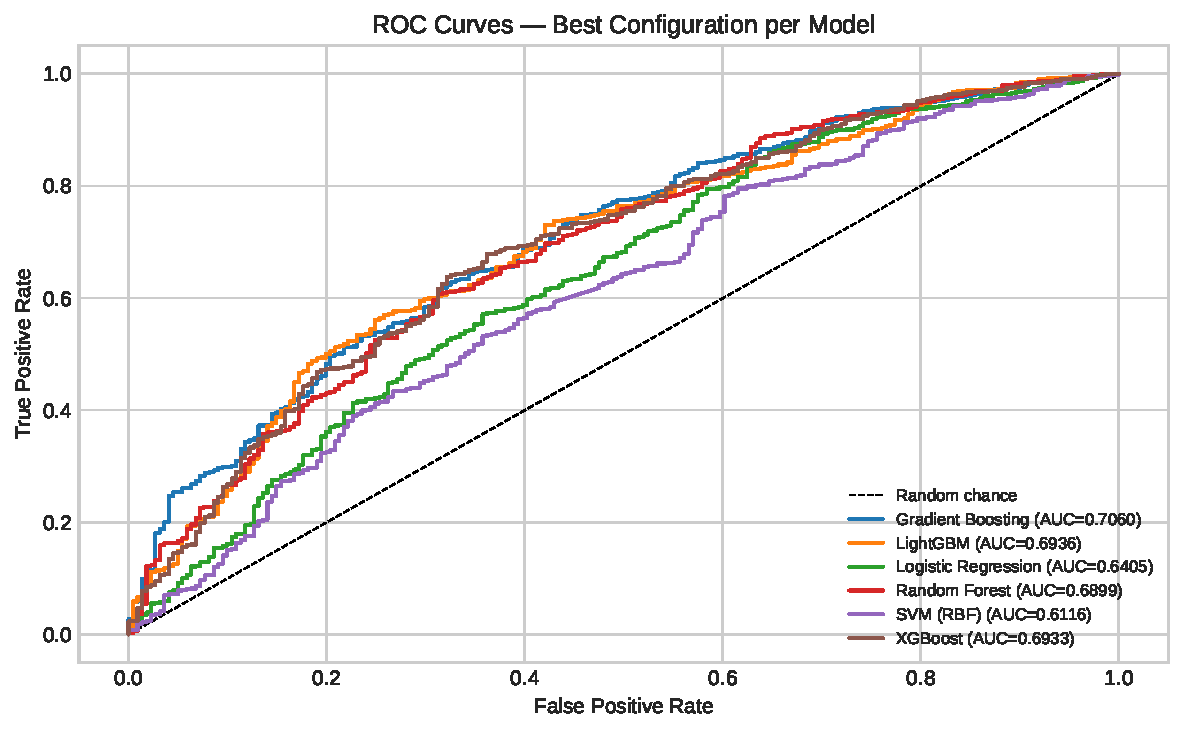
\includegraphics[width=\columnwidth]{figures/fig_roc_curves.pdf}
  \caption{Receiver Operating Characteristic (ROC) Curves for the Best Configuration per Algorithm on the Held-Out Test Set}
  \label{fig:roc_curves}
\end{figure}

\begin{figure}[htbp]
  \centering
  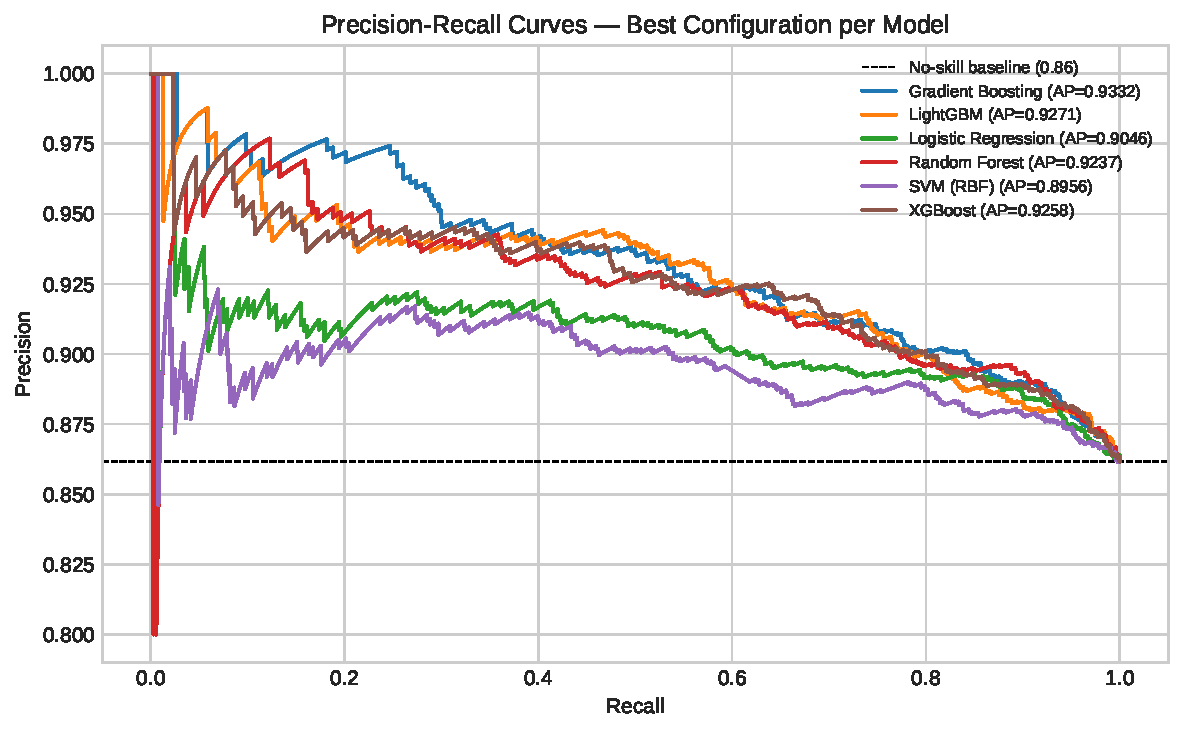
\includegraphics[width=\columnwidth]{figures/fig_pr_curves.pdf}
  \caption{Precision-Recall Curves for the Best Configuration per Algorithm (Dashed Baseline = Observed Failure Prevalence)}
  \label{fig:pr_curves}
\end{figure}

\FloatBarrier

Figure~\ref{fig:confusion_matrix} presents the confusion matrix of the best overall model on the test set, with cell values annotated as raw counts and row-normalized percentages, providing a direct view of misclassification patterns. Figure~\ref{fig:cv_boxplot} visualizes the distribution of five-fold stratified cross-validation ROC-AUC values across all experimental runs per algorithm, enabling a comparison of model stability in addition to mean performance.

\begin{figure}[htbp]
  \centering
  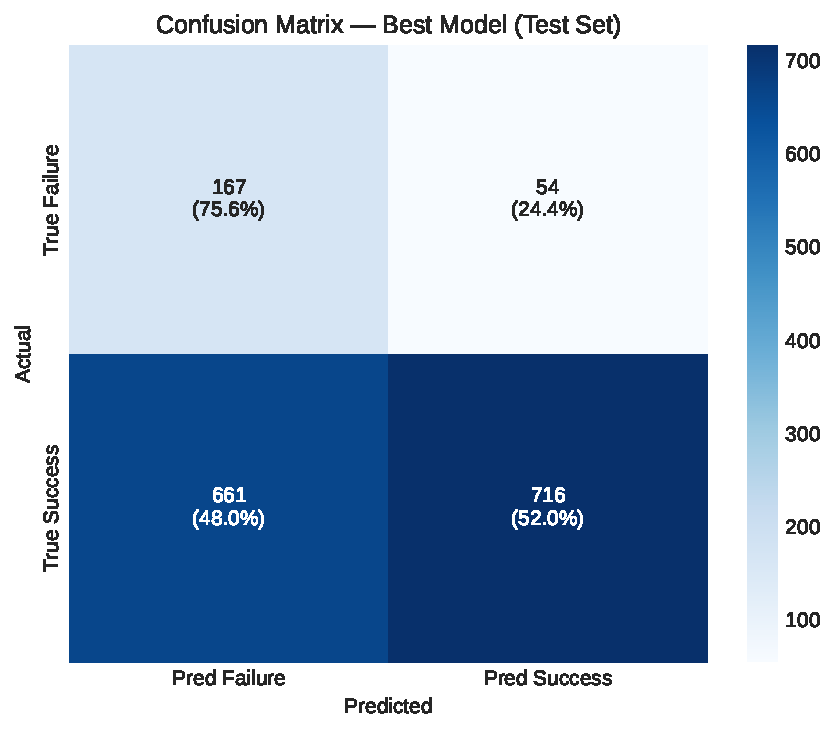
\includegraphics[width=0.7\columnwidth]{figures/fig_confusion_matrix.pdf}
  \caption{Confusion Matrix for the Best Overall Model on the Test Set (Annotated With Counts and Row-Normalized Percentages)}
  \label{fig:confusion_matrix}
\end{figure}

\begin{figure}[htbp]
  \centering
  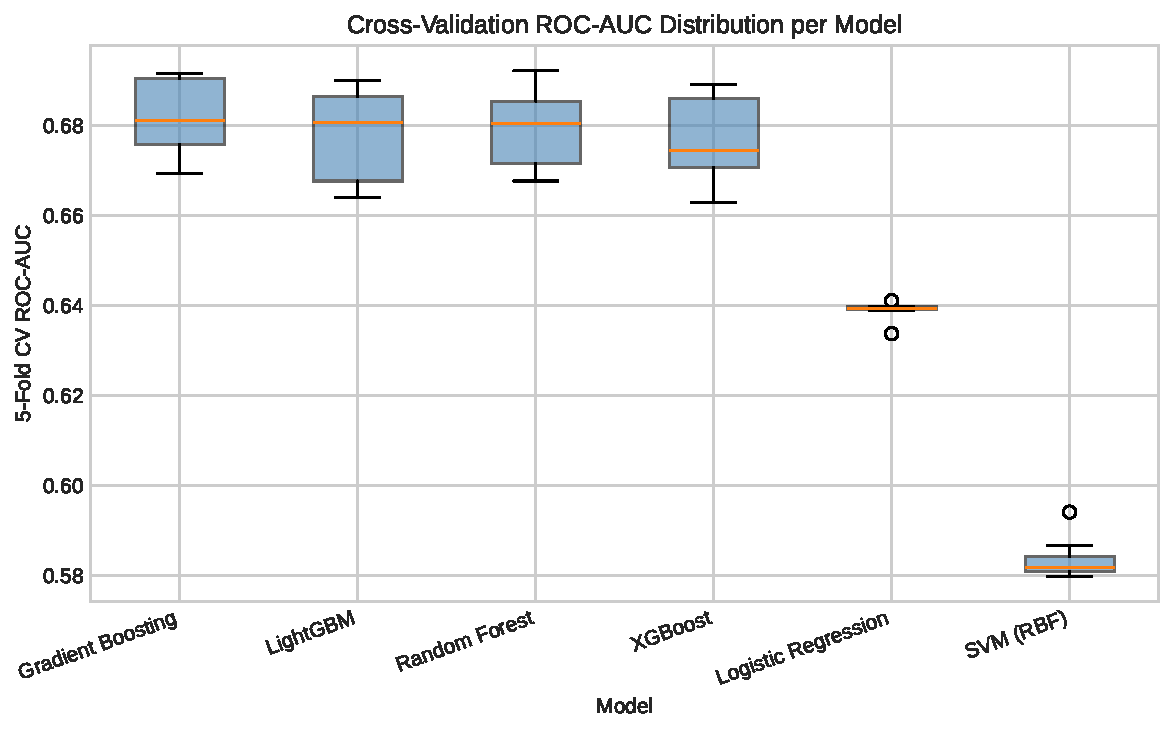
\includegraphics[width=\columnwidth]{figures/fig_cv_boxplot.pdf}
  \caption{Distribution of Five-Fold Stratified Cross-Validation ROC-AUC by Algorithm Across All Experimental Configurations}
  \label{fig:cv_boxplot}
\end{figure}

\FloatBarrier

Figure~\ref{fig:feature_importance} presents the top 15 normalized feature importances for the best overall model. These importances complement the SHAP-based interpretability described in the Supervised Learning subsection by providing a global ranking of predictor influence derived directly from the model's internal structure.

\begin{figure}[htbp]
  \centering
  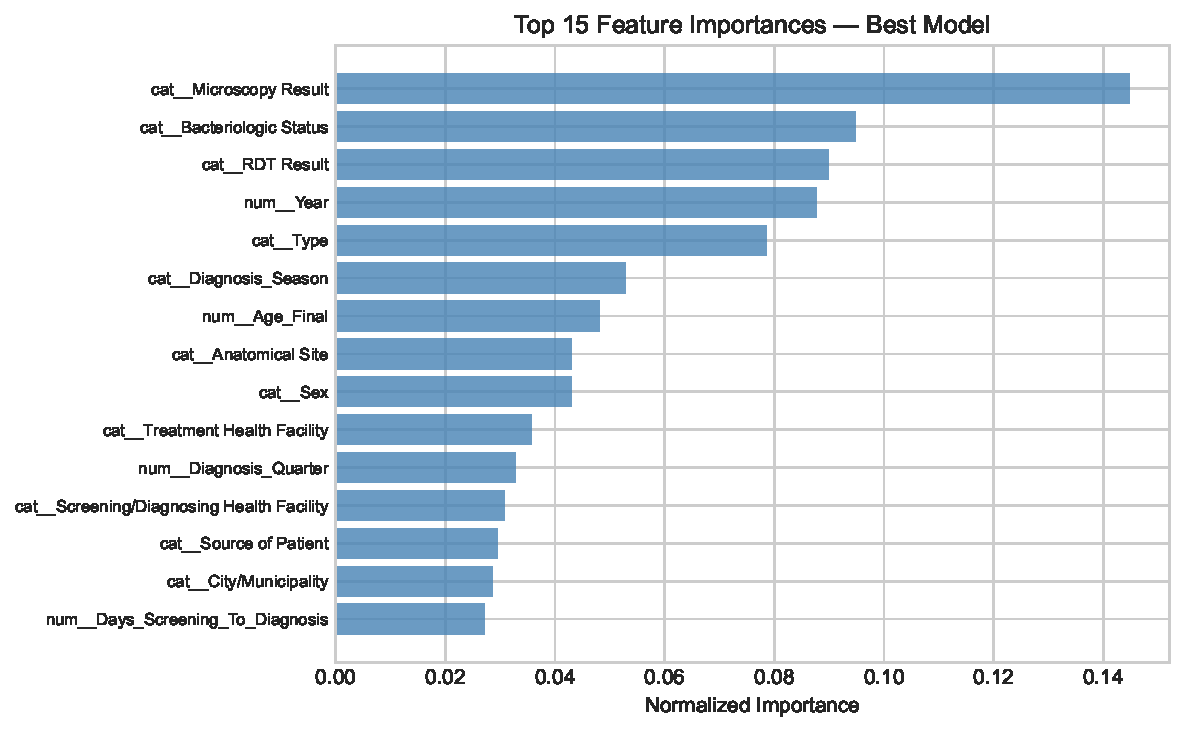
\includegraphics[width=\columnwidth]{figures/fig_feature_importance.pdf}
  \caption{Top 15 Normalized Feature Importances for the Best Overall Model}
  \label{fig:feature_importance}
\end{figure}

\FloatBarrier

\subsection{Temporal Models Performance}

\begin{table}[htbp]
\caption{Test Set Performance Metrics of Temporal Models for TB Treatment Outcome Prediction}
\label{tab:temporal_performance}
\resizebox{\columnwidth}{!}{%
\begin{tabular}{lcccccc}
\toprule
Metric & Bi-LSTM Baseline & Bi-LSTM Augmented & XGBoost Baseline & XGBoost SMOTE-ENN & LightGBM SMOTE-ENN & Random Forest SMOTE-ENN \\
\midrule
Accuracy & 0.9048 & 0.9048 & 0.9048 & 0.9048 & 0.9048 & 0.7143 \\
Precision & 0.9048 & 0.9048 & 0.9048 & 0.9048 & 0.9048 & 0.8824 \\
Recall & 1.0000 & 1.0000 & 1.0000 & 1.0000 & 1.0000 & 0.7895 \\
F1 Score & 0.9500 & 0.9500 & 0.9500 & 0.9500 & 0.9500 & 0.8333 \\
Specificity & 0.0000 & 0.0000 & 0.0000 & 0.0000 & 0.0000 & 0.0000 \\
ROC-AUC & 0.4737 & 0.3684 & 0.5789 & 0.1053 & 0.2105 & 0.5263 \\
PR-AUC & 0.8847 & 0.9099 & 0.9501 & 0.8356 & 0.8500 & 0.9419 \\
Threshold & 0.15 & 0.86 & 0.10 & 0.34 & 0.43 & 0.70 \\
\bottomrule
\end{tabular}%
}
\end{table}

Table \ref{tab:temporal_performance} presents the performance metrics of all temporal models evaluated on the held-out test set. Both Bi-LSTM variants and XGBoost Baseline achieved the highest overall accuracy (0.9048) and F1 score (0.9500), reflecting their ability to correctly predict the dominant Success class. Precision values were similarly high (0.9048), indicating few false positives for the majority class. However, recall for the minority Failure class reached 1.0 for these models, while specificity remained 0.0, demonstrating that no actual Failure cases were correctly identified in the small test set. Tree-based models augmented with SMOTE-ENN, particularly Random Forest, showed a more balanced performance. Random Forest achieved slightly lower overall accuracy (0.7143) but higher recall for the Failure class (0.7895) and competitive PR-AUC (0.9419), indicating better identification of high-risk patients. ROC-AUC scores further illustrate differences in probability calibration, with XGBoost Baseline achieving the highest ROC-AUC (0.5789), while the Bi-LSTM Augmented variant performed lower (0.3684), likely due to overfitting on limited Failure samples. Overall, these results suggest that while Bi-LSTM and XGBoost excel at predicting the majority outcome, Random Forest with SMOTE-ENN offers the most effective detection of treatment failure, making it more suitable for clinical decision support applications.

% ======================== DISCUSSION ========================
\section{Discussion}

This study investigated the use of machine learning models to predict treatment outcomes---Success or Failure---of PTB patients under the DOH-CAR TB-DOTS program, using monthly patient monitoring data alongside baseline clinical features. Both temporal models, specifically the Bi-LSTM Baseline and Augmented variants, and tree-based models, including XGBoost, LightGBM, and Random Forest with SMOTE-ENN, were evaluated on a stratified 70/20/10 patient-level split, incorporating progressive temporal samples from treatment months M0 through M12. The test set performance revealed that while Bi-LSTM and XGBoost Baseline models achieved high overall accuracy (0.9048) and F1 scores (0.9500), their ability to detect treatment failures was limited, as indicated by zero specificity for the minority Failure class. In contrast, Random Forest with SMOTE-ENN demonstrated more balanced performance, achieving a recall of 0.7895 for treatment failure and a high PR-AUC (0.9419), indicating greater reliability in identifying patients at risk of adverse outcomes. These results highlight that tree-based models augmented with SMOTE-ENN are particularly effective at handling severe class imbalance, while temporal models provide strong predictive accuracy for the majority outcome.

The study contributes in several ways. By integrating temporal monitoring data with static baseline features, it demonstrates that patient-level longitudinal information improves predictive performance over static data alone. The application of SMOTE-ENN and advanced data augmentation techniques for Bi-LSTM effectively addresses the extreme class imbalance inherent in TB treatment outcomes, enhancing the model's capacity to detect high-risk patients. Furthermore, the findings suggest that predictive models, particularly Random Forest with SMOTE-ENN, have practical value for clinical decision support systems, enabling clinicians to identify patients at risk of treatment failure early and prioritize interventions accordingly.

Based on these findings, it is recommended that healthcare facilities and policymakers consider integrating machine learning models like Random Forest with SMOTE-ENN into existing TB monitoring programs to improve treatment outcomes and optimize resource allocation. Future research should focus on larger, multi-region datasets to enhance generalization, explore hybrid modeling approaches combining deep learning and tree-based methods, and investigate additional features such as social determinants of health and geographic risk factors. Additionally, enhancing model interpretability, particularly of Bi-LSTM attention outputs, could improve clinician trust and adoption.

% ======================== ACKNOWLEDGMENTS ========================
\section{Acknowledgments}

The authors would like to express their sincere gratitude to Saint Louis University for providing the academic environment and resources that made this research possible. We extend our appreciation to the School of Accountancy, Management, Computing, and Information Studies (SAMCIS), specifically the Department of Computing and Information Studies, for their continuous support and guidance throughout the study. Our deepest thanks go to Dr. Randy Domantay, whose leadership and encouragement have been invaluable. We are especially grateful to our research adviser, Dr. Josephine S. Dela Cruz, for their expert guidance, insightful feedback, and unwavering support at every stage of the research. Lastly, we acknowledge the collaboration and contributions of our partner researchers from the SONAHBS Department of Pharmacy, whose expertise and assistance significantly enriched this study.

% ======================== REFERENCES ========================
% APA 7th: References heading is centered, bold, on its own page
\newpage
% apacite automatically formats the References heading;
% if it appears incorrectly, uncomment the next line:
% \section*{References}
\bibliography{references}

% ======================== APPENDICES ======================== TODO: fix spacing, there should be no space between the section heading and the pdf file
\newpage
\appendix

\section{Appendix A: iCreate Supplementary Material}
\label{app:supplementary}
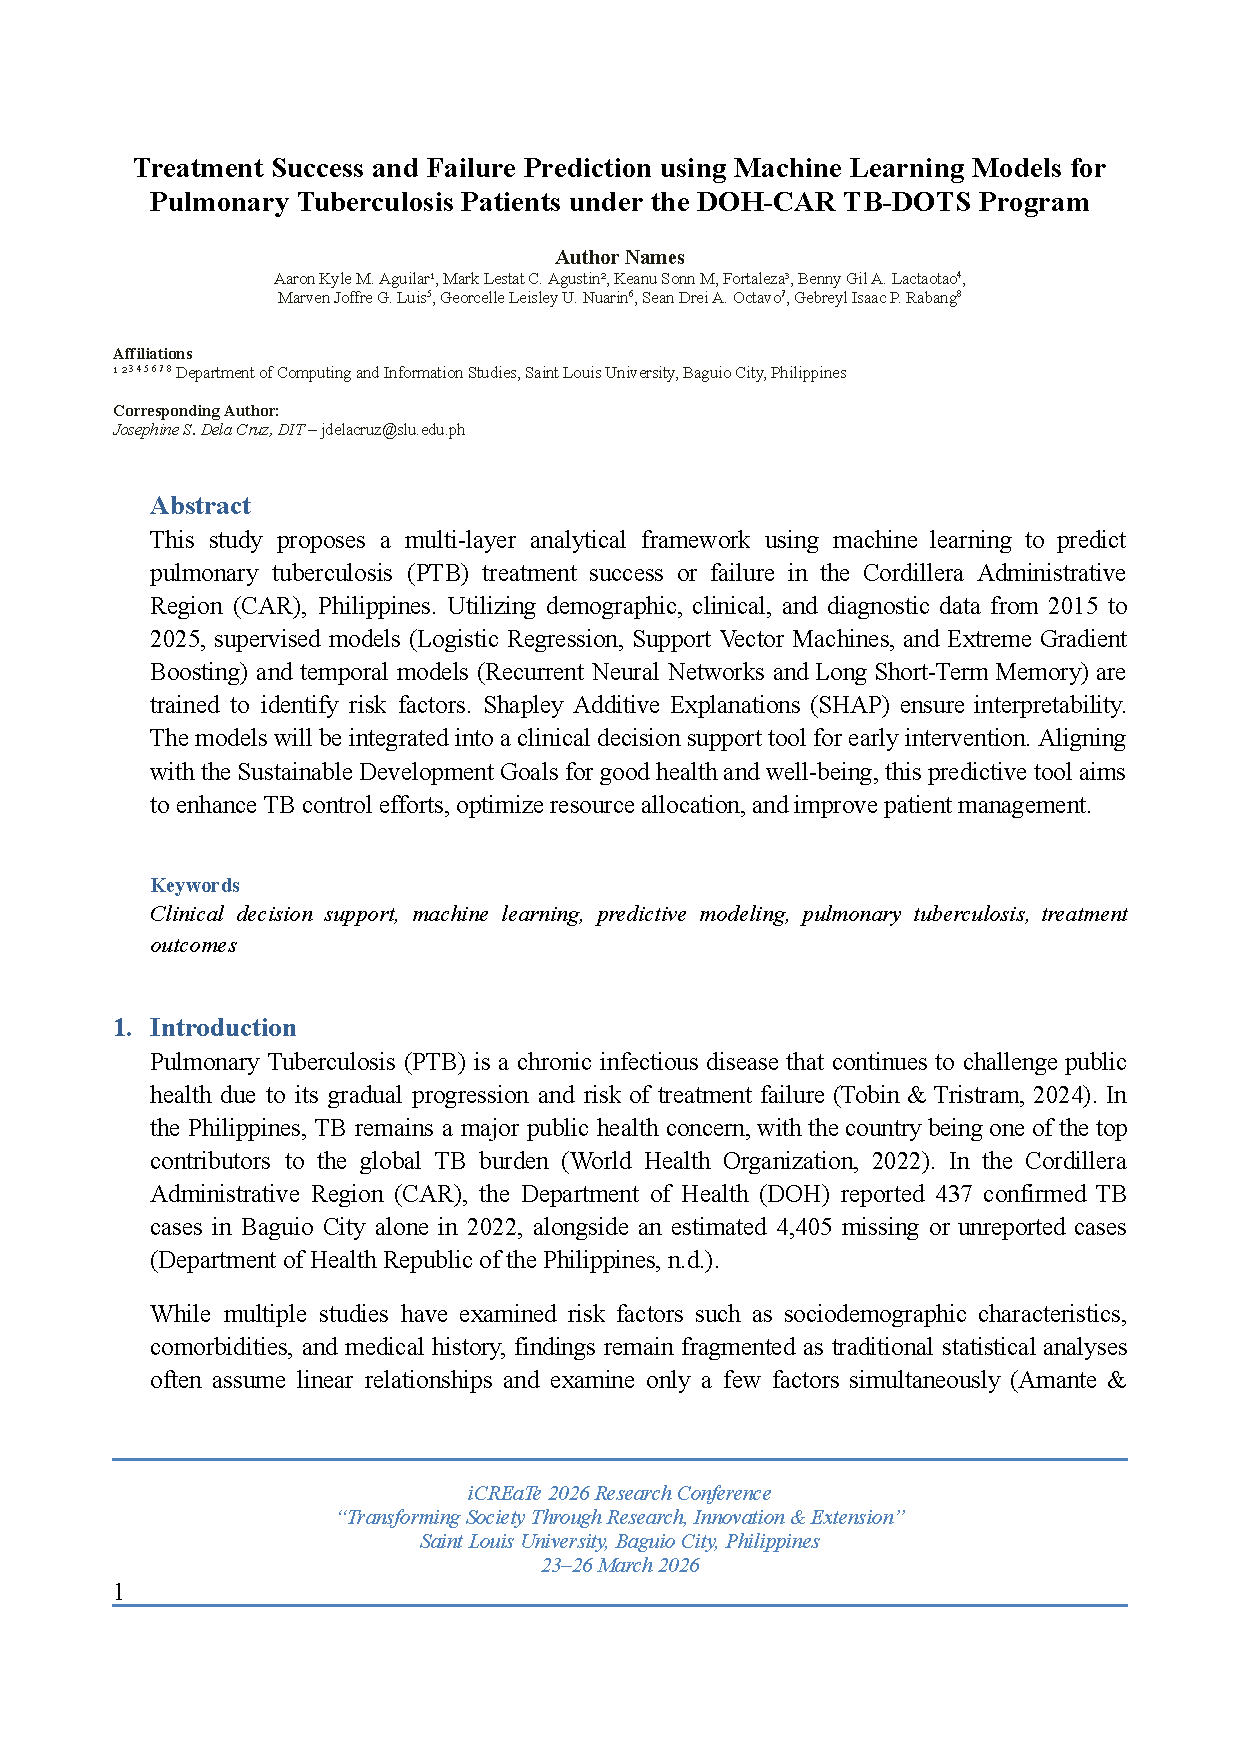
\includepdf[pages=-,pagecommand={\thispagestyle{fancy}}]{iCreate.pdf}


\end{document}
